\chapter{Phản xạ toàn phần}
\section{Lý thuyết trọng tâm}
\subsection{Hiện tượng phản xạ toàn phần}
\subsubsection{Định nghĩa}
Phản xạ toàn phần là hiện tượng phản xạ toàn bộ ánh sáng tới, xảy ra ở mặt phân cách giữa hai môi trường trong suốt.
\begin{center}
	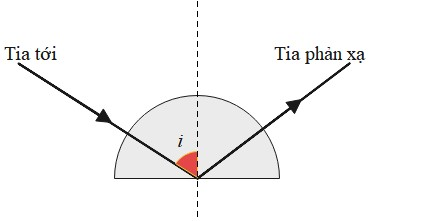
\includegraphics[scale=0.8]{../figs/VN11-PH-35-L-024-1-h60.jpg}
\end{center}
\subsubsection{Góc giới hạn phản xạ toàn phần}
\begin{center}
	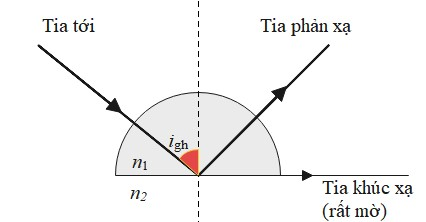
\includegraphics[scale=0.8]{../figs/VN11-PH-35-L-024-1-h59.jpg}
\end{center}
Góc giới hạn phản xạ toàn phần được tính theo công thức:
\begin{equation}
\sin i_{\text{gh}}=\dfrac{n_2}{n_1},
\end{equation}
trong đó,
\begin{itemize}
	\item $n_2$ là chiết suất của môi trường chiết quang hơn.
	\item $n_1$ là chiết suất của môi trường chiết quang kém.
	\item $ i_{\text{gh}}$ là góc giới hạn phản xạ toàn phần.
\end{itemize}
\subsubsection{Điều kiện để có phản xạ toàn phần}

\begin{itemize}
	\item Ánh sáng truyền từ một môi trường tới  môi trường chiết quang kém hơn.
	\begin{equation}
	n_1>n_2
	\end{equation}
	
	\item Góc tới lớn hơn hoặc bằng góc giới hạn.
		\begin{equation}
	i\geq i_{\text{gh}}
	\end{equation}
	
\end{itemize}

\subsection{Ứng dụng của hiện tượng phản xạ toàn phần: Cáp quang}
\subsubsection{Cấu tạo}
Cáp quang là bó sợi quang. Mỗi sợi quang là một dây trong suốt có tính dẫn sáng nhờ phản xạ toàn phần.

Sợi quang có lỏi làm bằng thủy tinh siêu sạch có chiết suất lớn $n_1$  được bao quanh bởi một lớp vỏ có chiết suất $n_2$ nhỏ hơn $n_1$. 

Phản xạ toàn phần xảy ra ở mặt phân cách giữa lõi và vỏ làm cho ánh sáng truyền đi được theo sợi quang. 

Ngoài cùng là một lớp võ bọc bằng nhựa dẻo để tạo cho cáp có độ bền và độ dai cơ học.

\subsubsection{Công dụng}
Cáp quang được ứng dụng vào việc truyền thông tin với nhiều ưu điểm: dung lượng tín hiệu lớn; nhỏ và nhẹ, dễ vận chuyển, dễ uốn; không bị nhiễu bởi các bức xạ điện từ bên ngoài; không có rủi ro cháy (vì không có dòng điện).

Trong y học, người ta dùng cáp quang để nội soi.


\section{Bài tập }
\begin{dang}{Góc giới hạn phản xạ toàn phần}
\end{dang}
\textbf{Phương pháp giải}

Sử dụng công thức tính góc giới hạn phản xạ toàn phần:
\begin{equation}
\sin i_{\text{gh}}=\dfrac{n_2}{n_1},
\end{equation}

Điều kiện xảy ra hiện tượng phàn xạ toàn phần
	\begin{eqnarray}
		n_1&>&n_2\\
		i&\geq& i_{\text{gh}}
	\end{eqnarray}

\vspace{1em}
\viduii{2}{
Biết chiết suất của thủy tinh là $\text{1,5}$; của nước là  $\dfrac{4}{3}$. Góc giới hạn phản xạ toàn phần khi ánh sáng truyền từ thủy tinh sang không khí, từ nước sang không khí và từ thủy tinh sang nước lần lượt là 

\begin{mcq}(2)
	\item $\text{41,8}^\circ; \ \text{48,6}^\circ; \ \text{62,7}^\circ$.
	\item $\text{48,6}^\circ; \ \text{41,8}^\circ; \ \text{62,7}^\circ$.
	\item $\text{62,7}^\circ; \ \text{48,6}^\circ; \ \text{41,8}^\circ$.
	\item $\text{62,7}^\circ; \ \text{41,8}^\circ; \ \text{48,6}^\circ$.
\end{mcq}}{
\begin{center}
	\textbf{Hướng dẫn giải:}
\end{center}

{Công thức góc giới hạn phản xạ toàn phần :
$\sin i_{\text{gh}}=\dfrac{n_2}{n_1}$.
\begin{itemize}
	\item Khi ánh sáng truyền từ thủy tinh sang không khí: $\sin i_\text{gh}=\dfrac{n_2}{n_1}=\dfrac{n_{\text{không khí}}}{n_{\text{thủy tinh}}}=\dfrac{1}{\text{1,5}}\Rightarrow i_\text{gh}\approx \text{41,8}^\circ$.
	\item Khi ánh sáng truyền từ nước sang không khí: $\sin i_\text{gh}=\dfrac{n_2}{n_1}=\dfrac{n_{\text{không khí}}}{n_{\text{nước}}}=\dfrac{1}{4/3}\Rightarrow i_\text{gh}\approx \text{48,6}^\circ$.
	\item  Khi ánh sáng truyền từ thủy tinh sang nước: $\sin i_\text{gh}=\dfrac{n_2}{n_1}=\dfrac{n_{\text{nước}}}{n_{\text{thủy tinh}}}=\dfrac{4/3}{\text{1,5}}\Rightarrow i_\text{gh}\approx \text{62,7}^\circ$.
\end{itemize}

\textbf{	Đáp án: A.}
}}

\viduii{2}{
Cho hai môi trường trong suốt là thủy tinh và không khí. Biết chiết suất của thủy tinh là $\text{1,5}$, chiết suất của không khí là 1. Để xảy ra hiện tượng phản xạ toàn phần, ta phải truyền ánh sáng như thế nào và góc giới hạn phản xạ toàn phần là bao nhiêu?

\begin{mcq}
	\item Ánh sáng từ không khí sang thủy tinh, góc giới hạn phản xạ toàn phần là $\text{41,8}^\circ$. 
	\item Ánh sáng từ thủy tinh sang không khí, góc giới hạn phản xạ toàn phần là $\text{41,8}^\circ$. 
	\item Ánh sáng từ không khí sang thủy tinh, góc giới hạn phản xạ toàn phần là $\text{62,7}^\circ$. 
	\item Ánh sáng từ thủy tinh sang không khí, góc giới hạn phản xạ toàn phần là $\text{62,7}^\circ$. 
\end{mcq}}{
\begin{center}
	\textbf{Hướng dẫn giải:}
\end{center}

{Điều kiện xảy ra hiện tượng phản xạ toàn phần là ánh sáng truyền từ một môi trường tới  môi trường chiết quang kém hơn. Do đó, ánh sáng phải truyền truyền từ thủy tinh sang không khí.
	
$\sin i_\text{gh}=\dfrac{n_2}{n_1}=\dfrac{n_{\text{không khí}}}{n_{\text{thủy tinh}}}=\dfrac{1}{\text{1,5}}\Rightarrow i_\text{gh}\approx \text{41,8}^\circ$.

\textbf{	Đáp án: B.}
	}
}

\viduii{2}
{Một ngọn đèn nhỏ S đặt ở đáy một bể nước $\left( n=\dfrac{4}{3}\right) $, độ cao mực nước $h=60\ \text{cm}$. Bán kính nhỏ nhất của tấm gỗ tròn nổi trên mặt nước sao cho không một tia sáng nào từ S lọt ra ngoài không khí là
\begin{center}
	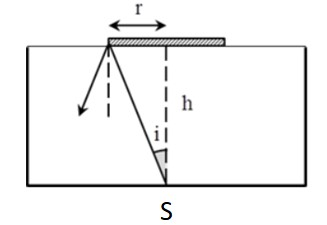
\includegraphics[scale=0.8]{../figs/VN11-PH-35-L-024-1-h61.jpg}
\end{center}
\begin{mcq}(4)
	\item $49\ \text{cm}$.
	\item $55\ \text{cm}$.
	\item $68\ \text{cm}$. 
	\item $51\ \text{cm}$. 
\end{mcq}}
{\begin{center}
	\textbf{Hướng dẫn giải:}
\end{center}

	$\sin i_\text{gh}=\dfrac{n_2}{n_1}=\dfrac{n_{\text{không khí}}}{n_{\text{nước}}}=\dfrac{1}{\text{4/3}}\Rightarrow i_\text{gh}\approx \text{48,6}^\circ$.
	
	Để không có tia sáng nào từ S lọt ra không khí thì $i\geq i_{\text{gh}}$.
	
	Khi đó: $\tan i_{\text{min}}=\tan i_{\text{gh}}=\dfrac{r_\text{min}}{h}\Rightarrow r_\text{min}=h\cdot \tan i_{\text{gh}}=68\ \text{cm}$.
	
\textbf{	Đáp án: C.}

}
\viduii{3}
{Một sợi quang hình trụ gồm phần lõi có chiết suất $n=\text{1,60}$ và phần vỏ bọc có chiết suất $n_0=\text{1,41}$. Trong không khí, một tia sáng tới mặt trước của sợi quang tại điểm O (O nằm trên trục của sợi quang) với góc tới $\alpha$ rồi khúc xạ vào phần lõi (như hình bên). Để tia sáng chỉ truyền trong phần lõi thì giá trị lớn nhất của góc $\alpha$ gần nhất với giá trị nào sau đây?
\begin{center}
	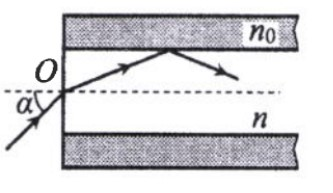
\includegraphics[scale=0.6]{../figs/VN11-PH-35-L-024-1-h62.jpg}
\end{center}
\begin{mcq}(4)
	\item $\text{38}^\circ$.
	\item $\text{45}^\circ$.
	\item $\text{49}^\circ$.
	\item $\text{33}^\circ$. 
\end{mcq}}
{\begin{center}
	\textbf{Hướng dẫn giải:}
\end{center}

Gọi $\beta$ là góc tới khi tia sáng đến chỗ tiếp giáp giữa phần lõi và phần vỏ bọc. 

Công thức định luật khúc xạ ánh sáng: $\dfrac{\sin \alpha }{\sin \left(90^\circ-\beta \right)}=n$.

$\Rightarrow \dfrac{\sin \alpha }{\cos \beta }=n$
$\Rightarrow \dfrac{\sin \alpha }{\sqrt{1-\sin^2\beta} }=n$
$\Rightarrow \sin^2\beta=1-\dfrac{\sin^2 \alpha }{n^2}$.

Điều kiện phản xạ toàn phần: $\sin \beta\geq \dfrac{n_0}{n}$.

$\Rightarrow 1-\dfrac{\sin^2 \alpha }{n^2}\geq \dfrac{n^2_0}{n^2}$.

$\Rightarrow \sin \alpha \leq \sqrt{n^2-n^2_0}$.

$\Rightarrow \alpha_\text{max} =\text{49,13}^\circ$.

Vậy $\alpha$ gần nhất với giá trị $\text{49}^\circ$.

\textbf{Đáp án: C.}

}

